%----------------------------------------------------------------------------------------
%    PACKAGES AND THEMES
%----------------------------------------------------------------------------------------
\documentclass[aspectratio=169,xcolor=dvipsnames]{beamer}
\makeatletter
\def\input@path{{../BeamerTemplate/theme/}}
\makeatother
\usetheme{CleanEasy}
\usepackage[utf8]{inputenc}
\usepackage{lmodern}
\usepackage[T1]{fontenc}
\usepackage{fix-cm}
\usepackage{amsmath}
\usepackage{mathtools}
\usepackage{listings}
\usepackage{xcolor}
\usepackage{hyperref}
\usepackage{graphicx}
\usepackage{booktabs}
\usepackage{tikz}
\usetikzlibrary{positioning, shapes, arrows, calc, decorations.pathreplacing, arrows.meta, backgrounds, patterns, overlay-beamer-styles}
\usepackage{etoolbox}
\usepackage{multirow}

%----------------------------------------------------------------------------------------
%    LAYOUT CONFIGURATION
%----------------------------------------------------------------------------------------
\input{../BeamerTemplate/configs/configs}

%----------------------------------------------------------------------------------------
%    TITLE PAGE CONFIGURATION
%----------------------------------------------------------------------------------------
\title[Linear Data Structures]{Linear Data Structures}
\author{Minseok Jeon}
\institute{DGIST}
\date{\today}

% Simple title page without logos
\titlegraphic{}

%----------------------------------------------------------------------------------------

\begin{document}

\begin{frame}[plain]
  \titlepage
\end{frame}

\begin{frame}[plain]{Contents}
  \tableofcontents
\end{frame}

%----------------------------------------------------------------------------------------
%    INTRODUCTION
%----------------------------------------------------------------------------------------
\section{Introduction}

\begin{frame}{What Are Linear Data Structures?}
  \begin{definition}
    \textbf{Linear data structures} are structures where elements are arranged \textbf{sequentially}, with each element having at most one predecessor and one successor.
  \end{definition}

  \vspace{0.5cm}

  \begin{columns}
    \begin{column}{0.48\textwidth}
      \textbf{Covered Structures:}
      \begin{itemize}
        \item Arrays (Static \& Dynamic)
        \item Linked Lists (Singly, Doubly, Circular)
        \item Stacks (LIFO)
        \item Queues (FIFO)
        \item Deques \& Circular Queues
        \item Priority Queues
      \end{itemize}
    \end{column}
    \begin{column}{0.48\textwidth}
      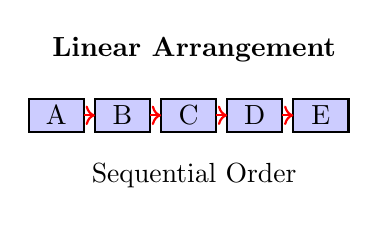
\begin{tikzpicture}[scale=0.7]
        \node at (3,3.5) {\textbf{Linear Arrangement}};

        % Sequential elements
        \foreach \i/\val in {0/A, 1/B, 2/C, 3/D, 4/E} {
          \draw[thick, fill=blue!20] (\i*1.2,2) rectangle (\i*1.2+1,2.6);
          \node at (\i*1.2+0.5,2.3) {\val};
        }

        % Arrows showing sequence
        \foreach \i in {0,1,2,3} {
          \draw[->, thick, red] (\i*1.2+1,2.3) -- (\i*1.2+1.2,2.3);
        }

        \node[below] at (3,1.6) {Sequential Order};
      \end{tikzpicture}
    \end{column}
  \end{columns}

  \vspace{0.5cm}

  \begin{alertblock}{Key Characteristic}
    Elements can be traversed in a single direction (or bidirectionally in some cases), making them ideal for sequential processing.
  \end{alertblock}
\end{frame}

%----------------------------------------------------------------------------------------
%    ARRAYS
%----------------------------------------------------------------------------------------
\section{Arrays}

\begin{frame}{Arrays: The Foundation}
  \begin{definition}
    An \textbf{array} is a contiguous block of memory storing elements of the same type in sequential memory locations, providing \textbf{O(1) indexing}.
  \end{definition}

  \vspace{0.3cm}

  \begin{columns}
    \begin{column}{0.55\textwidth}
      \textbf{Key Properties:}
      \begin{itemize}
        \item Contiguous memory allocation
        \item Direct access by index
        \item Fixed or dynamic size
        \item Cache-friendly (spatial locality)
      \end{itemize}

      \vspace{0.3cm}

      \begin{exampleblock}{Memory Address}
        \texttt{addr[i] = base + i × sizeof(element)}
      \end{exampleblock}
    \end{column}
    \begin{column}{0.4\textwidth}
      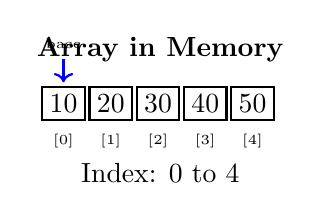
\begin{tikzpicture}[scale=0.6]
        \node at (2.5,4) {\textbf{Array in Memory}};

        \foreach \i/\val in {0/10, 1/20, 2/30, 3/40, 4/50} {
          \draw[thick] (\i*1,2.5) rectangle (\i*1+0.9,3.2);
          \node at (\i*1+0.45,2.85) {\val};
          \node[below] at (\i*1+0.45,2.4) {\tiny[\i]};
        }

        \draw[->, thick, blue] (0.45,3.8) -- (0.45,3.3);
        \node[above] at (0.45,3.8) {\tiny base};

        \node[below] at (2.5,1.8) {Index: 0 to 4};
      \end{tikzpicture}
    \end{column}
  \end{columns}
\end{frame}

\begin{frame}{Static vs Dynamic Arrays}
  \begin{columns}
    \begin{column}{0.48\textwidth}
      \begin{block}{Static Arrays}
        \textbf{Fixed size at creation}

        \vspace{0.2cm}

        Pros:
        \begin{itemize}
          \item[$\checkmark$] No resize overhead
          \item[$\checkmark$] Predictable memory
          \item[$\checkmark$] Slightly faster
        \end{itemize}

        \vspace{0.2cm}

        Cons:
        \begin{itemize}
          \item[$\times$] Cannot grow/shrink
          \item[$\times$] Must know size
          \item[$\times$] Wasted or insufficient space
        \end{itemize}
      \end{block}

      \vspace{0.2cm}

      \begin{exampleblock}{Examples}
        C: \texttt{int arr[100];} \\
        Java: \texttt{int[] arr = new int[100];}
      \end{exampleblock}
    \end{column}
    \begin{column}{0.48\textwidth}
      \begin{block}{Dynamic Arrays}
        \textbf{Resizable as needed}

        \vspace{0.2cm}

        Pros:
        \begin{itemize}
          \item[$\checkmark$] Flexible size
          \item[$\checkmark$] O(1) amortized append
          \item[$\checkmark$] No size constraints
        \end{itemize}

        \vspace{0.2cm}

        Cons:
        \begin{itemize}
          \item[$\times$] Occasional resize (O(n))
          \item[$\times$] Extra capacity overhead
          \item[$\times$] Unpredictable resizing
        \end{itemize}
      \end{block}

      \vspace{0.2cm}

      \begin{exampleblock}{Examples}
        Python: \texttt{list} \\
        C++: \texttt{std::vector} \\
        Java: \texttt{ArrayList}
      \end{exampleblock}
    \end{column}
  \end{columns}
\end{frame}

\begin{frame}[fragile]{Dynamic Array Growth Strategy}
  \begin{columns}
    \begin{column}{0.55\textwidth}
      \textbf{How It Works:}
      \begin{enumerate}
        \item Start with small capacity (e.g., 4)
        \item When full, allocate new array (2× size)
        \item Copy all elements to new array
        \item Free old array
      \end{enumerate}

      \vspace{0.3cm}

      \begin{exampleblock}{Growth Sequence}
        Capacity: 1 → 2 → 4 → 8 → 16 → 32 ...
      \end{exampleblock}

      \vspace{0.3cm}

      \begin{alertblock}{Amortized O(1)}
        For n insertions: \\
        Total copies = 1 + 2 + 4 + ... + n = 2n - 1 \\
        Average: (2n - 1)/n $\approx$ 2 = O(1)
      \end{alertblock}
    \end{column}
    \begin{column}{0.4\textwidth}
      \begin{exampleblock}{Python Example}
        \begin{lstlisting}[language=Python,basicstyle=\tiny\ttfamily]
class DynamicArray:
    def __init__(self):
        self._capacity = 4
        self._size = 0
        self._data = [None] * 4

    def append(self, item):
        if self._size == self._capacity:
            self._resize(2 * self._capacity)
        self._data[self._size] = item
        self._size += 1

    def _resize(self, new_cap):
        new_data = [None] * new_cap
        for i in range(self._size):
            new_data[i] = self._data[i]
        self._data = new_data
        self._capacity = new_cap
        \end{lstlisting}
      \end{exampleblock}
    \end{column}
  \end{columns}
\end{frame}

\begin{frame}{Array Performance Summary}
  \begin{center}
    \begin{tabular}{l|c|c|p{4cm}}
      \toprule
      \textbf{Operation} & \textbf{Static} & \textbf{Dynamic} & \textbf{Notes} \\
      \midrule
      Access by index & O(1) & O(1) & Direct memory access \\
      Search (unsorted) & O(n) & O(n) & Linear scan \\
      Search (sorted) & O(log n) & O(log n) & Binary search \\
      Insert at end & N/A & O(1) amortized & May trigger resize \\
      Insert at middle & O(n) & O(n) & Shift elements \\
      Delete & O(n) & O(n) & Shift elements \\
      Memory usage & Exact & Extra capacity & ~25-50\% overhead \\
      \bottomrule
    \end{tabular}
  \end{center}

  \vspace{0.5cm}

  \begin{block}{When to Use Arrays}
    \begin{itemize}
      \item Need fast random access by index
      \item Size is known or changes infrequently
      \item Mostly reading data, few insertions/deletions
      \item Want cache-friendly performance
    \end{itemize}
  \end{block}
\end{frame}

%----------------------------------------------------------------------------------------
%    LINKED LISTS
%----------------------------------------------------------------------------------------
\section{Linked Lists}

\begin{frame}{Introduction to Linked Lists}
  \begin{definition}
    A \textbf{linked list} is a linear structure where elements (nodes) are stored non-contiguously in memory. Each node contains data and a reference (pointer) to the next node.
  \end{definition}

  \vspace{0.3cm}

  \begin{columns}
    \begin{column}{0.55\textwidth}
      \textbf{Key Differences from Arrays:}
      \begin{itemize}
        \item[$\times$] No random access (must traverse)
        \item[$\checkmark$] Dynamic size (no preallocation)
        \item[$\checkmark$] O(1) insert/delete at known position
        \item[$\times$] Extra memory for pointers
        \item[$\times$] Poor cache locality
      \end{itemize}
    \end{column}
    \begin{column}{0.4\textwidth}
      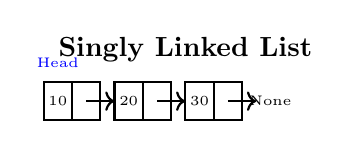
\begin{tikzpicture}[scale=0.6]
        \node at (3,3.5) {\textbf{Singly Linked List}};

        % Nodes
        \draw[thick] (0,2) rectangle (0.6,2.8);
        \draw[thick] (0.6,2) rectangle (1.2,2.8);
        \node at (0.3,2.4) {\tiny 10};
        \draw[->, thick] (0.9,2.4) -- (1.5,2.4);

        \draw[thick] (1.5,2) rectangle (2.1,2.8);
        \draw[thick] (2.1,2) rectangle (2.7,2.8);
        \node at (1.8,2.4) {\tiny 20};
        \draw[->, thick] (2.4,2.4) -- (3,2.4);

        \draw[thick] (3,2) rectangle (3.6,2.8);
        \draw[thick] (3.6,2) rectangle (4.2,2.8);
        \node at (3.3,2.4) {\tiny 30};
        \draw[->, thick] (3.9,2.4) -- (4.5,2.4);

        \node at (4.8,2.4) {\tiny None};

        \node[above, blue] at (0.3,2.9) {\tiny Head};
      \end{tikzpicture}
    \end{column}
  \end{columns}
\end{frame}

\begin{frame}{Types of Linked Lists}
  \begin{columns}
    \begin{column}{0.32\textwidth}
      \begin{block}{Singly Linked}
        Each node points to next only

        \vspace{0.2cm}

        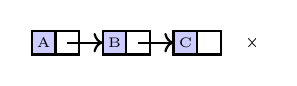
\begin{tikzpicture}[scale=0.5]
          \foreach \i/\val in {0/A, 1/B, 2/C} {
            \draw[thick, fill=blue!20] (\i*1.8,0) rectangle (\i*1.8+0.6,0.6);
            \draw[thick] (\i*1.8+0.6,0) rectangle (\i*1.8+1.2,0.6);
            \node at (\i*1.8+0.3,0.3) {\tiny\val};
            \ifnum\i<2
              \draw[->, thick] (\i*1.8+0.9,0.3) -- (\i*1.8+1.8,0.3);
            \fi
          }
          \node at (5.6,0.3) {\tiny ×};
        \end{tikzpicture}

        \vspace{0.2cm}

        Memory: 1 pointer/node \\
        Traverse: Forward only
      \end{block}
    \end{column}
    \begin{column}{0.32\textwidth}
      \begin{block}{Doubly Linked}
        Pointers to next \& prev

        \vspace{0.2cm}

        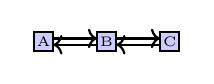
\begin{tikzpicture}[scale=0.4]
          \foreach \i/\val in {0/A, 1/B, 2/C} {
            \draw[thick, fill=blue!20] (\i*2,0) rectangle (\i*2+0.6,0.6);
            \node at (\i*2+0.3,0.3) {\tiny\val};
            \ifnum\i<2
              \draw[->, thick] (\i*2+0.6,0.4) -- (\i*2+2,0.4);
              \draw[<-, thick] (\i*2+0.6,0.2) -- (\i*2+2,0.2);
            \fi
          }
        \end{tikzpicture}

        \vspace{0.2cm}

        Memory: 2 pointers/node \\
        Traverse: Both directions
      \end{block}
    \end{column}
    \begin{column}{0.32\textwidth}
      \begin{block}{Circular}
        Last points to first

        \vspace{0.2cm}

        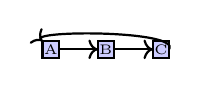
\begin{tikzpicture}[scale=0.35]
          \foreach \i/\val in {0/A, 1/B, 2/C} {
            \draw[thick, fill=blue!20] (\i*2,0) rectangle (\i*2+0.6,0.6);
            \node at (\i*2+0.3,0.3) {\tiny\val};
            \ifnum\i<2
              \draw[->, thick] (\i*2+0.6,0.3) -- (\i*2+2,0.3);
            \fi
          }
          \draw[->, thick] (4.6,0.3) .. controls (5,1) and (-0.5,1) .. (0,0.6);
        \end{tikzpicture}

        \vspace{0.2cm}

        Forms a circle \\
        No NULL end
      \end{block}
    \end{column}
  \end{columns}

  \vspace{0.5cm}

  \begin{center}
    \begin{tabular}{l|c|c|c}
      \toprule
      \textbf{Feature} & \textbf{Singly} & \textbf{Doubly} & \textbf{Circular} \\
      \midrule
      Memory/node & 1 pointer & 2 pointers & 1-2 pointers \\
      Forward traverse & \checkmark & \checkmark & \checkmark \\
      Backward traverse & × & \checkmark & × (singly) \\
      Insert at beginning & O(1) & O(1) & O(1) \\
      Insert at end & O(n) or O(1)* & O(1) & O(n) or O(1)* \\
      \bottomrule
    \end{tabular}
  \end{center}

  \tiny{*O(1) with tail pointer}
\end{frame}

\begin{frame}[fragile]{Singly Linked List Implementation}
  \begin{columns}
    \begin{column}{0.48\textwidth}
      \begin{exampleblock}{Node Class}
        \begin{lstlisting}[language=Python,basicstyle=\tiny\ttfamily]
class Node:
    def __init__(self, data):
        self.data = data
        self.next = None
        \end{lstlisting}
      \end{exampleblock}

      \begin{exampleblock}{Insert at Beginning}
        \begin{lstlisting}[language=Python,basicstyle=\tiny\ttfamily]
def insert_at_beginning(self, data):
    new_node = Node(data)
    new_node.next = self.head
    self.head = new_node
    self.size += 1
# O(1) - just update head
        \end{lstlisting}
      \end{exampleblock}
    \end{column}
    \begin{column}{0.48\textwidth}
      \begin{exampleblock}{Insert at End}
        \begin{lstlisting}[language=Python,basicstyle=\tiny\ttfamily]
def insert_at_end(self, data):
    new_node = Node(data)
    if not self.head:
        self.head = new_node
    else:
        current = self.head
        while current.next:  # O(n)
            current = current.next
        current.next = new_node
    self.size += 1
        \end{lstlisting}
      \end{exampleblock}

      \begin{exampleblock}{Delete Node}
        \begin{lstlisting}[language=Python,basicstyle=\tiny\ttfamily]
def delete(self, data):
    if self.head.data == data:
        self.head = self.head.next
        return True

    current = self.head
    while current.next:
        if current.next.data == data:
            current.next = current.next.next
            return True
        current = current.next
    return False
        \end{lstlisting}
      \end{exampleblock}
    \end{column}
  \end{columns}
\end{frame}

\begin{frame}{Linked List vs Array}
  \begin{center}
    \begin{tabular}{l|c|c}
      \toprule
      \textbf{Operation} & \textbf{Array} & \textbf{Linked List} \\
      \midrule
      Access by index & O(1) & O(n) \\
      Search & O(n) & O(n) \\
      Insert at beginning & O(n) & O(1) \\
      Insert at end & O(1) amortized & O(n) or O(1)* \\
      Insert at middle & O(n) & O(1)** \\
      Delete at beginning & O(n) & O(1) \\
      Delete at middle & O(n) & O(1)** \\
      Memory overhead & Low & High (pointers) \\
      Cache performance & Excellent & Poor \\
      \bottomrule
    \end{tabular}
  \end{center}

  \tiny{*O(1) with tail pointer, **If position is known}

  \vspace{0.5cm}

  \begin{columns}
    \begin{column}{0.48\textwidth}
      \begin{block}{Use Arrays When}
        \begin{itemize}
          \item Need random access
          \item Size known/stable
          \item Mostly reading
          \item Want cache performance
        \end{itemize}
      \end{block}
    \end{column}
    \begin{column}{0.48\textwidth}
      \begin{block}{Use Linked Lists When}
        \begin{itemize}
          \item Frequent insertions/deletions
          \item Size unknown/dynamic
          \item No random access needed
          \item Memory fragmentation OK
        \end{itemize}
      \end{block}
    \end{column}
  \end{columns}
\end{frame}

%----------------------------------------------------------------------------------------
%    STACKS
%----------------------------------------------------------------------------------------
\section{Stacks}

\begin{frame}{Stacks: LIFO Principle}
  \begin{definition}
    A \textbf{stack} is a linear data structure following \textbf{LIFO} (Last In, First Out). The last element added is the first one removed, like a stack of plates.
  \end{definition}

  \vspace{0.3cm}

  \begin{columns}
    \begin{column}{0.55\textwidth}
      \textbf{Core Operations (All O(1)):}
      \begin{itemize}
        \item \texttt{push(item)}: Add to top
        \item \texttt{pop()}: Remove from top
        \item \texttt{peek()}: View top without removing
        \item \texttt{is\_empty()}: Check if empty
        \item \texttt{size()}: Get element count
      \end{itemize}

      \vspace{0.3cm}

      \begin{alertblock}{Key Restriction}
        Only the \textbf{top} element is accessible. This restriction is intentional and enables many algorithms.
      \end{alertblock}
    \end{column}
    \begin{column}{0.4\textwidth}
      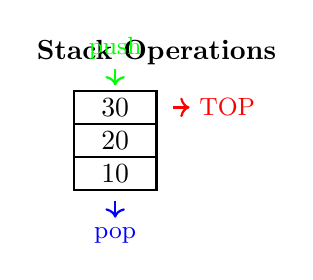
\begin{tikzpicture}[scale=0.7]
        \node at (2,4.5) {\textbf{Stack Operations}};

        % Stack
        \draw[thick] (0.5,2) rectangle (2,2.6);
        \draw[thick] (0.5,2.6) rectangle (2,3.2);
        \draw[thick] (0.5,3.2) rectangle (2,3.8);

        \node at (1.25,2.3) {10};
        \node at (1.25,2.9) {20};
        \node at (1.25,3.5) {30};

        \draw[->, thick, red] (2.3,3.5) -- (2.6,3.5);
        \node[right, red] at (2.6,3.5) {\small TOP};

        \draw[->, thick, green] (1.25,4.2) -- (1.25,3.9);
        \node[above, green] at (1.25,4.2) {\small push};

        \draw[->, thick, blue] (1.25,1.8) -- (1.25,1.5);
        \node[below, blue] at (1.25,1.5) {\small pop};
      \end{tikzpicture}
    \end{column}
  \end{columns}
\end{frame}

\begin{frame}[fragile]{Stack Implementations}
  \begin{columns}
    \begin{column}{0.48\textwidth}
      \begin{exampleblock}{Array-Based Stack}
        \begin{lstlisting}[language=Python,basicstyle=\tiny\ttfamily]
class ArrayStack:
    def __init__(self):
        self._data = []

    def push(self, item):
        self._data.append(item)  # O(1)

    def pop(self):
        if self.is_empty():
            raise IndexError("empty")
        return self._data.pop()  # O(1)

    def peek(self):
        if self.is_empty():
            raise IndexError("empty")
        return self._data[-1]  # O(1)

    def is_empty(self):
        return len(self._data) == 0

    def size(self):
        return len(self._data)
        \end{lstlisting}
      \end{exampleblock}
    \end{column}
    \begin{column}{0.48\textwidth}
      \begin{exampleblock}{Linked List-Based Stack}
        \begin{lstlisting}[language=Python,basicstyle=\tiny\ttfamily]
class LinkedStack:
    def __init__(self):
        self._head = None
        self._size = 0

    def push(self, item):
        new_node = Node(item)
        new_node.next = self._head
        self._head = new_node
        self._size += 1  # O(1)

    def pop(self):
        if self.is_empty():
            raise IndexError("empty")
        item = self._head.data
        self._head = self._head.next
        self._size -= 1
        return item  # O(1)

    def peek(self):
        if self.is_empty():
            raise IndexError("empty")
        return self._head.data

    def is_empty(self):
        return self._head is None
        \end{lstlisting}
      \end{exampleblock}
    \end{column}
  \end{columns}
\end{frame}

\begin{frame}[fragile]{Stack Applications}
  \begin{columns}
    \begin{column}{0.48\textwidth}
      \begin{exampleblock}{1. Function Call Stack}
        \begin{lstlisting}[language=Python,basicstyle=\tiny\ttfamily]
def factorial(n):
    if n <= 1:
        return 1
    return n * factorial(n - 1)

# Call stack for factorial(3):
# factorial(3)
#   factorial(2)
#     factorial(1) <- TOP
#       returns 1
#     returns 2
#   returns 6
        \end{lstlisting}
      \end{exampleblock}

      \begin{exampleblock}{2. Balanced Parentheses}
        \begin{lstlisting}[language=Python,basicstyle=\tiny\ttfamily]
def is_balanced(expr):
    stack = []
    pairs = {'(':')', '[':']', '{':'}'}

    for char in expr:
        if char in pairs:
            stack.append(char)
        elif char in pairs.values():
            if not stack or \
               pairs[stack.pop()] != char:
                return False
    return len(stack) == 0

# "([{}])" -> True
# "([)]"   -> False
        \end{lstlisting}
      \end{exampleblock}
    \end{column}
    \begin{column}{0.48\textwidth}
      \begin{exampleblock}{3. Undo/Redo}
        \begin{lstlisting}[language=Python,basicstyle=\tiny\ttfamily]
class TextEditor:
    def __init__(self):
        self.text = ""
        self.undo_stack = []
        self.redo_stack = []

    def write(self, text):
        self.undo_stack.append(self.text)
        self.text += text
        self.redo_stack.clear()

    def undo(self):
        if self.undo_stack:
            self.redo_stack.append(
                self.text)
            self.text = \
                self.undo_stack.pop()

    def redo(self):
        if self.redo_stack:
            self.undo_stack.append(
                self.text)
            self.text = \
                self.redo_stack.pop()
        \end{lstlisting}
      \end{exampleblock}

      \begin{block}{Other Uses}
        \begin{itemize}
          \item Expression evaluation
          \item DFS traversal
          \item Backtracking algorithms
          \item Browser history
        \end{itemize}
      \end{block}
    \end{column}
  \end{columns}
\end{frame}

%----------------------------------------------------------------------------------------
%    QUEUES
%----------------------------------------------------------------------------------------
\section{Queues}

\begin{frame}{Queues: FIFO Principle}
  \begin{definition}
    A \textbf{queue} is a linear data structure following \textbf{FIFO} (First In, First Out). The first element added is the first one removed, like a waiting line.
  \end{definition}

  \vspace{0.3cm}

  \begin{columns}
    \begin{column}{0.55\textwidth}
      \textbf{Core Operations (All O(1)):}
      \begin{itemize}
        \item \texttt{enqueue(item)}: Add to rear
        \item \texttt{dequeue()}: Remove from front
        \item \texttt{front()}: View front without removing
        \item \texttt{is\_empty()}: Check if empty
        \item \texttt{size()}: Get element count
      \end{itemize}

      \vspace{0.3cm}

      \begin{alertblock}{Key Property}
        Fair processing: first come, first served
      \end{alertblock}
    \end{column}
    \begin{column}{0.4\textwidth}
      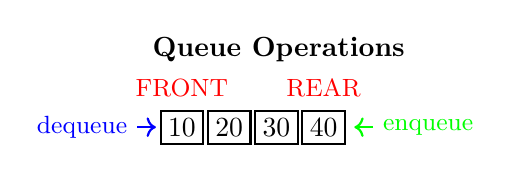
\begin{tikzpicture}[scale=0.6]
        \node at (2.5,3.5) {\textbf{Queue Operations}};

        % Queue
        \foreach \i/\val in {0/10, 1/20, 2/30, 3/40} {
          \draw[thick] (\i*1,1.5) rectangle (\i*1+0.9,2.2);
          \node at (\i*1+0.45,1.85) {\val};
        }

        \draw[->, thick, blue] (-0.5,1.85) -- (-0.1,1.85);
        \node[left, blue] at (-0.5,1.85) {\small dequeue};

        \draw[->, thick, green] (4.5,1.85) -- (4.1,1.85);
        \node[right, green] at (4.5,1.85) {\small enqueue};

        \node[above, red] at (0.45,2.3) {\small FRONT};
        \node[above, red] at (3.45,2.3) {\small REAR};
      \end{tikzpicture}
    \end{column}
  \end{columns}
\end{frame}

\begin{frame}[fragile]{Queue Implementations}
  \begin{columns}
    \begin{column}{0.48\textwidth}
      \begin{alertblock}{Naive (Bad!)}
        \begin{lstlisting}[language=Python,basicstyle=\tiny\ttfamily]
class NaiveQueue:
    def __init__(self):
        self._data = []

    def enqueue(self, item):
        self._data.append(item)  # O(1)

    def dequeue(self):
        return self._data.pop(0)  # O(n)!
        # Shifts all elements left!
        \end{lstlisting}
      \end{alertblock}

      \begin{exampleblock}{Using Deque (Good!)}
        \begin{lstlisting}[language=Python,basicstyle=\tiny\ttfamily]
from collections import deque

class Queue:
    def __init__(self):
        self._data = deque()

    def enqueue(self, item):
        self._data.append(item)  # O(1)

    def dequeue(self):
        if self.is_empty():
            raise IndexError("empty")
        return self._data.popleft()  # O(1)

    def front(self):
        return self._data[0]
        \end{lstlisting}
      \end{exampleblock}
    \end{column}
    \begin{column}{0.48\textwidth}
      \begin{exampleblock}{Linked List Queue}
        \begin{lstlisting}[language=Python,basicstyle=\tiny\ttfamily]
class LinkedQueue:
    def __init__(self):
        self._head = None
        self._tail = None
        self._size = 0

    def enqueue(self, item):
        new_node = Node(item)
        if self._tail is None:
            self._head = self._tail = \
                new_node
        else:
            self._tail.next = new_node
            self._tail = new_node
        self._size += 1  # O(1)

    def dequeue(self):
        if self.is_empty():
            raise IndexError("empty")
        item = self._head.data
        self._head = self._head.next
        if self._head is None:
            self._tail = None
        self._size -= 1
        return item  # O(1)
        \end{lstlisting}
      \end{exampleblock}
    \end{column}
  \end{columns}
\end{frame}

\begin{frame}[fragile]{Queue Applications}
  \begin{columns}
    \begin{column}{0.48\textwidth}
      \begin{exampleblock}{1. Task Scheduling}
        \begin{lstlisting}[language=Python,basicstyle=\tiny\ttfamily]
class TaskScheduler:
    def __init__(self):
        self.queue = Queue()

    def add_task(self, task):
        self.queue.enqueue(task)

    def process_next(self):
        if not self.queue.is_empty():
            task = self.queue.dequeue()
            print(f"Processing: {task}")

# First added = first processed
        \end{lstlisting}
      \end{exampleblock}

      \begin{exampleblock}{2. Print Queue}
        \begin{lstlisting}[language=Python,basicstyle=\tiny\ttfamily]
class PrintQueue:
    def __init__(self):
        self.queue = Queue()

    def add_document(self, doc):
        self.queue.enqueue(doc)

    def print_next(self):
        if not self.queue.is_empty():
            doc = self.queue.dequeue()
            print(f"Printing: {doc}")
        \end{lstlisting}
      \end{exampleblock}
    \end{column}
    \begin{column}{0.48\textwidth}
      \begin{exampleblock}{3. BFS Traversal}
        \begin{lstlisting}[language=Python,basicstyle=\tiny\ttfamily]
def bfs(graph, start):
    visited = set()
    queue = Queue()
    queue.enqueue(start)
    visited.add(start)

    while not queue.is_empty():
        node = queue.dequeue()
        print(node)

        for neighbor in graph[node]:
            if neighbor not in visited:
                visited.add(neighbor)
                queue.enqueue(neighbor)

# Explores level by level
        \end{lstlisting}
      \end{exampleblock}

      \begin{block}{Other Uses}
        \begin{itemize}
          \item Request handling (web servers)
          \item Message queues
          \item Buffering (streaming)
          \item Simulation systems
        \end{itemize}
      \end{block}
    \end{column}
  \end{columns}
\end{frame}

%----------------------------------------------------------------------------------------
%    DEQUE AND CIRCULAR QUEUE
%----------------------------------------------------------------------------------------
\section{Deque \& Circular Queue}

\begin{frame}[fragile]{Deque (Double-Ended Queue)}
  \begin{definition}
    A \textbf{deque} (pronounced "deck") allows insertion and deletion at \textbf{both ends} (front and rear). It combines capabilities of stacks and queues.
  \end{definition}

  \vspace{0.3cm}

  \begin{columns}
    \begin{column}{0.55\textwidth}
      \textbf{Operations (All O(1)):}
      \begin{itemize}
        \item \texttt{add\_front(item)}
        \item \texttt{add\_rear(item)}
        \item \texttt{remove\_front()}
        \item \texttt{remove\_rear()}
        \item \texttt{front()}, \texttt{rear()}
      \end{itemize}

      \vspace{0.3cm}

      \begin{exampleblock}{Python Implementation}
        \begin{lstlisting}[language=Python,basicstyle=\tiny\ttfamily]
from collections import deque

dq = deque()
dq.appendleft(10)   # add_front
dq.append(20)       # add_rear
dq.popleft()        # remove_front
dq.pop()            # remove_rear
        \end{lstlisting}
      \end{exampleblock}
    \end{column}
    \begin{column}{0.4\textwidth}
      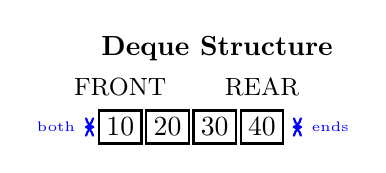
\begin{tikzpicture}[scale=0.6]
        \node at (2.5,3.5) {\textbf{Deque Structure}};

        \foreach \i/\val in {0/10, 1/20, 2/30, 3/40} {
          \draw[thick] (\i*1,1.5) rectangle (\i*1+0.9,2.2);
          \node at (\i*1+0.45,1.85) {\val};
        }

        \draw[<->, thick, blue] (-0.3,1.85) -- (-0.1,1.85);
        \node[left, blue] at (-0.3,1.85) {\tiny both};

        \draw[<->, thick, blue] (4.1,1.85) -- (4.3,1.85);
        \node[right, blue] at (4.3,1.85) {\tiny ends};

        \node[above] at (0.45,2.3) {\small FRONT};
        \node[above] at (3.45,2.3) {\small REAR};
      \end{tikzpicture}

      \vspace{0.3cm}

      \begin{block}{Use Cases}
        \begin{itemize}
          \item Palindrome checking
          \item Sliding window problems
          \item Browser history (fast back/forward)
          \item Work stealing queues
        \end{itemize}
      \end{block}
    \end{column}
  \end{columns}
\end{frame}

\begin{frame}{Circular Queue}
  \begin{definition}
    A \textbf{circular queue} reuses empty spaces when elements are dequeued. The rear wraps around to the beginning when it reaches the end.
  \end{definition}

  \vspace{0.3cm}

  \begin{columns}
    \begin{column}{0.55\textwidth}
      \textbf{Why Circular?}
      \begin{itemize}
        \item Regular queue: empty spaces at front wasted
        \item Circular queue: reuses freed space
        \item Fixed capacity (efficient for buffers)
      \end{itemize}

      \vspace{0.3cm}

      \begin{exampleblock}{Key Formula}
        \texttt{rear = (front + size) \% capacity} \\
        \texttt{front = (front + 1) \% capacity}
      \end{exampleblock}

      \vspace{0.3cm}

      \begin{block}{Applications}
        \begin{itemize}
          \item CPU scheduling (round-robin)
          \item Streaming buffers
          \item Traffic light systems
          \item Memory management
        \end{itemize}
      \end{block}
    \end{column}
    \begin{column}{0.4\textwidth}
      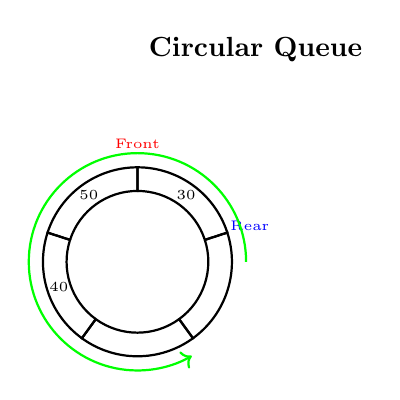
\begin{tikzpicture}[scale=0.6]
        \node at (2.5,4.5) {\textbf{Circular Queue}};

        % Circular representation
        \foreach \i/\val in {0/30, 1/, 2/, 3/40, 4/50} {
          \pgfmathsetmacro{\angle}{90 - \i*72}
          \draw[thick] (\angle:1.5) -- (\angle:2) arc (\angle:\angle-72:2) -- (\angle-72:1.5) arc (\angle-72:\angle:1.5);
          \node at (\angle-36:1.75) {\tiny\val};
        }

        % Labels
        \node[red] at (90:2.5) {\tiny Front};
        \node[blue] at (18:2.5) {\tiny Rear};

        % Circular arrow
        \draw[->, thick, green] (0:2.3) arc (0:300:2.3);
      \end{tikzpicture}

      \vspace{0.2cm}

      After dequeue twice, then enqueue(40,50): \\
      Rear wrapped around to use freed space!
    \end{column}
  \end{columns}
\end{frame}

%----------------------------------------------------------------------------------------
%    PRIORITY QUEUE
%----------------------------------------------------------------------------------------
\section{Priority Queue}

\begin{frame}[fragile]{Priority Queue Overview}
  \begin{definition}
    A \textbf{priority queue} is an ADT where each element has an associated \textbf{priority}. Elements with higher priority are dequeued first, regardless of insertion order.
  \end{definition}

  \vspace{0.3cm}

  \begin{columns}
    \begin{column}{0.55\textwidth}
      \textbf{Key Difference:}
      \begin{itemize}
        \item Regular queue: FIFO
        \item Priority queue: Highest priority first
      \end{itemize}

      \vspace{0.3cm}

      \textbf{Operations:}
      \begin{itemize}
        \item \texttt{insert(item, priority)}: O(log n)
        \item \texttt{extract\_min/max()}: O(log n)
        \item \texttt{peek()}: O(1)
      \end{itemize}

      \vspace{0.3cm}

      \begin{alertblock}{Implementation}
        Typically uses \textbf{binary heap} for O(log n) operations
      \end{alertblock}
    \end{column}
    \begin{column}{0.4\textwidth}
      \begin{exampleblock}{Visual Example}
        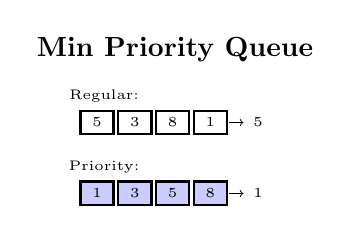
\begin{tikzpicture}[scale=0.6]
          \node at (2,4) {\textbf{Min Priority Queue}};

          % Regular queue
          \node at (0.5,3) {\tiny Regular:};
          \foreach \i/\val in {0/5, 1/3, 2/8, 3/1} {
            \draw[thick] (\i*0.8,2.2) rectangle (\i*0.8+0.7,2.7);
            \node at (\i*0.8+0.35,2.45) {\tiny\val};
          }
          \node at (3.5,2.45) {\tiny → 5};

          % Priority queue
          \node at (0.5,1.5) {\tiny Priority:};
          \foreach \i/\val in {0/1, 1/3, 2/5, 3/8} {
            \draw[thick, fill=blue!20] (\i*0.8,0.7) rectangle (\i*0.8+0.7,1.2);
            \node at (\i*0.8+0.35,0.95) {\tiny\val};
          }
          \node at (3.5,0.95) {\tiny → 1};
        \end{tikzpicture}
      \end{exampleblock}

      \vspace{0.3cm}

      \begin{exampleblock}{Python Usage}
        \begin{lstlisting}[language=Python,basicstyle=\tiny\ttfamily]
import heapq
heap = []
heapq.heappush(heap, (1, "High"))
heapq.heappush(heap, (5, "Low"))
item = heapq.heappop(heap)  # "High"
        \end{lstlisting}
      \end{exampleblock}
    \end{column}
  \end{columns}
\end{frame}

\begin{frame}[fragile]{Priority Queue Applications}
  \begin{columns}
    \begin{column}{0.48\textwidth}
      \begin{exampleblock}{1. Emergency Room}
        \begin{lstlisting}[language=Python,basicstyle=\tiny\ttfamily]
class EmergencyRoom:
    def __init__(self):
        self.queue = PriorityQueue()

    def admit_patient(self, name, severity):
        # Lower = more critical
        self.queue.insert(name, severity)

    def treat_next(self):
        # Treats most critical first
        return self.queue.extract_min()

er = EmergencyRoom()
er.admit_patient("Alice", 5)  # Minor
er.admit_patient("Bob", 1)    # Critical
er.treat_next()  # Bob (critical)
        \end{lstlisting}
      \end{exampleblock}

      \begin{exampleblock}{2. Task Scheduler}
        \begin{lstlisting}[language=Python,basicstyle=\tiny\ttfamily]
class TaskScheduler:
    def __init__(self):
        self.pq = PriorityQueue()

    def add_task(self, task, deadline):
        # Earlier deadline = higher priority
        self.pq.insert(task, deadline)

    def do_next_task(self):
        return self.pq.extract_min()
        \end{lstlisting}
      \end{exampleblock}
    \end{column}
    \begin{column}{0.48\textwidth}
      \begin{exampleblock}{3. Dijkstra's Algorithm}
        \begin{lstlisting}[language=Python,basicstyle=\tiny\ttfamily]
def dijkstra(graph, start):
    distances = {node: float('inf')
                 for node in graph}
    distances[start] = 0
    pq = PriorityQueue()
    pq.insert(start, 0)

    while not pq.is_empty():
        current = pq.extract_min()

        for neighbor, weight in \
                graph[current]:
            dist = distances[current] + \
                   weight
            if dist < distances[neighbor]:
                distances[neighbor] = dist
                pq.insert(neighbor, dist)

    return distances
        \end{lstlisting}
      \end{exampleblock}

      \begin{block}{Other Uses}
        \begin{itemize}
          \item Event-driven simulation
          \item Huffman coding
          \item A* pathfinding
          \item Median maintenance
        \end{itemize}
      \end{block}
    \end{column}
  \end{columns}
\end{frame}

%----------------------------------------------------------------------------------------
%    COMPARISON
%----------------------------------------------------------------------------------------
\section{Comparison \& Use Cases}

\begin{frame}{Performance Summary}
  \begin{center}
    \small
    \begin{tabular}{l|c|c|c|c|c|c}
      \toprule
      \textbf{Structure} & \textbf{Access} & \textbf{Insert (begin)} & \textbf{Insert (end)} & \textbf{Delete (begin)} & \textbf{Delete (end)} & \textbf{Search} \\
      \midrule
      Array & O(1) & O(n) & O(n) & O(n) & O(n) & O(n) \\
      Dynamic Array & O(1) & O(n) & O(1)* & O(n) & O(1) & O(n) \\
      Singly Linked & O(n) & O(1) & O(n)** & O(1) & O(n) & O(n) \\
      Doubly Linked & O(n) & O(1) & O(1) & O(1) & O(1) & O(n) \\
      Stack & N/A & O(1) & N/A & O(1) & N/A & N/A \\
      Queue & N/A & N/A & O(1) & O(1) & N/A & N/A \\
      Deque & N/A & O(1) & O(1) & O(1) & O(1) & N/A \\
      Priority Queue & N/A & O(log n) & O(log n) & O(log n) & N/A & O(n) \\
      \bottomrule
    \end{tabular}
  \end{center}

  \vspace{0.2cm}
  \tiny{*amortized, **O(1) with tail pointer}

  \vspace{0.5cm}

  \begin{block}{Memory Overhead Comparison}
    \begin{itemize}
      \item \textbf{Array}: Minimal (just elements) + potential unused capacity
      \item \textbf{Singly Linked List}: 1 pointer per node
      \item \textbf{Doubly Linked List}: 2 pointers per node
      \item \textbf{Circular Queue}: Fixed capacity array
    \end{itemize}
  \end{block}
\end{frame}

\begin{frame}{Decision Guide: Which Structure to Use?}
  \begin{center}
    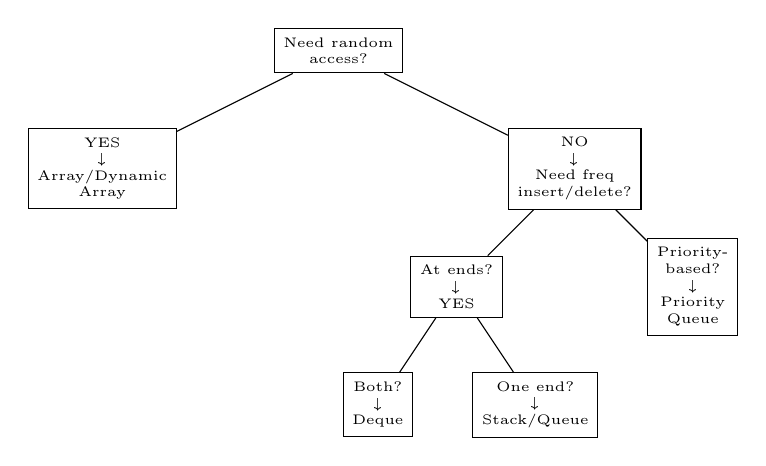
\begin{tikzpicture}[
      level 1/.style={sibling distance=6cm, level distance=1.5cm},
      level 2/.style={sibling distance=3cm, level distance=1.5cm},
      level 3/.style={sibling distance=2cm, level distance=1.5cm},
      every node/.style={rectangle, draw, align=center, font=\tiny}
    ]
      \node {Need random\\access?}
        child {node {YES\\↓\\Array/Dynamic\\Array}
        }
        child {node {NO\\↓\\Need freq\\insert/delete?}
          child {node {At ends?\\↓\\YES}
            child {node {Both?\\↓\\Deque}}
            child {node {One end?\\↓\\Stack/Queue}}
          }
          child {node {Priority-\\based?\\↓\\Priority\\Queue}}
        };
    \end{tikzpicture}
  \end{center}
\end{frame}

\begin{frame}{Real-World Use Cases}
  \begin{center}
    \begin{tabular}{p{4cm}|p{3cm}|p{4cm}}
      \toprule
      \textbf{Scenario} & \textbf{Structure} & \textbf{Reason} \\
      \midrule
      Student grades (by ID) & Dynamic Array & Fast access by index, known size \\
      \midrule
      Text editor undo/redo & Two Stacks & LIFO matches undo/redo behavior \\
      \midrule
      Web server requests & Queue & FIFO ensures fairness \\
      \midrule
      Music playlist & Doubly Linked List & Easy forward/backward, insert anywhere \\
      \midrule
      CPU scheduling & Priority Queue or Circular Queue & Priority-based or round-robin \\
      \midrule
      Browser history & Deque & Fast back/forward navigation \\
      \midrule
      Video streaming buffer & Circular Queue & Fixed buffer, continuous read/write \\
      \midrule
      Expression parser & Stack & Handle nested structures \\
      \midrule
      BFS graph traversal & Queue & Level-by-level exploration \\
      \midrule
      DFS graph traversal & Stack & Depth-first exploration \\
      \bottomrule
    \end{tabular}
  \end{center}
\end{frame}

\begin{frame}[fragile]{Common Mistakes to Avoid}
  \begin{alertblock}{1. Using \texttt{list.pop(0)} for Queue}
    \begin{lstlisting}[language=Python,basicstyle=\tiny\ttfamily]
# BAD: O(n) - shifts all elements!
queue = []
queue.append(1)
queue.pop(0)

# GOOD: O(1) with deque
from collections import deque
queue = deque()
queue.append(1)
queue.popleft()
    \end{lstlisting}
  \end{alertblock}

  \begin{alertblock}{2. Using Linked List for Random Access}
    \begin{lstlisting}[language=Python,basicstyle=\tiny\ttfamily]
# BAD: if you need frequent access by index
linked_list.get(100)  # O(n) traversal

# GOOD: use array
array[100]  # O(1)
    \end{lstlisting}
  \end{alertblock}

  \begin{alertblock}{3. Not Considering Cache Performance}
    \begin{itemize}
      \item Array: [1][2][3][4] - contiguous, excellent cache
      \item Linked List: scattered in memory, poor cache
      \item For large datasets, array can be 10-100× faster even with O(n) ops!
    \end{itemize}
  \end{alertblock}
\end{frame}

%----------------------------------------------------------------------------------------
%    SUMMARY
%----------------------------------------------------------------------------------------
\section{Summary}

\begin{frame}{Key Takeaways}
  \begin{block}{Arrays}
    \begin{itemize}
      \item O(1) access, cache-friendly, but O(n) insert/delete in middle
      \item Dynamic arrays: O(1) amortized append via doubling strategy
      \item Use when: need random access, size known/stable
    \end{itemize}
  \end{block}

  \begin{block}{Linked Lists}
    \begin{itemize}
      \item O(1) insert/delete at known positions, dynamic size
      \item Singly: 1 pointer, forward only; Doubly: 2 pointers, bidirectional
      \item Use when: frequent insertions/deletions, no random access needed
    \end{itemize}
  \end{block}

  \begin{block}{Stacks \& Queues}
    \begin{itemize}
      \item Stack (LIFO): function calls, undo, expression parsing, DFS
      \item Queue (FIFO): task scheduling, BFS, fair processing
      \item Deque: flexible both ends, palindromes, sliding windows
    \end{itemize}
  \end{block}

  \begin{block}{Priority Queue}
    \begin{itemize}
      \item Priority-based processing, O(log n) ops with heap
      \item Use when: need highest/lowest priority element quickly
      \item Applications: Dijkstra's, scheduling, event simulation
    \end{itemize}
  \end{block}
\end{frame}

\begin{frame}{Implementation Guidelines}
  \begin{block}{From Scratch vs Libraries}
    \textbf{Implement from scratch to learn:}
    \begin{itemize}
      \item Understand internal mechanisms
      \item Practice pointer manipulation
      \item Learn complexity trade-offs
    \end{itemize}

    \vspace{0.3cm}

    \textbf{Use library implementations for production:}
    \begin{itemize}
      \item Python: \texttt{list}, \texttt{collections.deque}, \texttt{heapq}
      \item C++: \texttt{std::vector}, \texttt{std::list}, \texttt{std::stack}, \texttt{std::queue}
      \item Java: \texttt{ArrayList}, \texttt{LinkedList}, \texttt{Stack}, \texttt{PriorityQueue}
    \end{itemize}
  \end{block}

  \vspace{0.3cm}

  \begin{alertblock}{Remember}
    \begin{itemize}
      \item Choose based on most frequent operations
      \item Consider cache performance for large datasets
      \item Test with realistic data sizes
      \item Profile before optimizing
    \end{itemize}
  \end{alertblock}
\end{frame}

\begin{frame}[plain]
  \begin{center}
    {\Huge Thank You!}

    \vspace{1cm}

    {\large Questions?}

    \vspace{1cm}

    \textit{``The right data structure makes the algorithm simple.\\
    The wrong data structure makes it impossible.''}
  \end{center}
\end{frame}

\end{document}
